\documentclass{article}
\usepackage[swedish]{babel}
\usepackage[utf8]{inputenc}
\usepackage{graphicx}
\usepackage{verbatim}
\usepackage{graphicx}
\title{
  Västtrafik Reviewer \\
  \large Projektarbete av grupp 8 i kurs ENM156, Hållbar utveckling och etik inom datateknik }
  
\author{Alaa Eddin Alasiri, Felix Bråberg, \\Linus Johansson, Oscar Lilja, Rik Muijs, Philip Vedin}
\date{November 2020}


%======================/SAKER SOM SKA VARA MED I RAPPORTEN\======================
\begin{comment}
Generellt:
-Referera till kurslitteratur inom kursen
-Målgrupp = andra studenter i kursen
-Mellan 6-9 sidor
-Reflekterande text tydligen

Element som ska vara med:
-En kort beskrivning av er applikation.
-Reflektion kopplat till hållbarhet och etik.
-Hur skulle ni kunna göra bättre?
-Vilka är egna lärdomar?

För att rapporten ska var godkänd krävs att:
• Alla fyra punkter från listan ovan finns redovisade i rapporten
• Ni använder på ett korrekt sätt begrepp och teorier om hållbar utveckling och etik som presenteras i kurslitteraturen och föreläsningarna
• Ni skriver utifrån er själva och era egna erfarenheter
• Ni reflekterar över grunder och konsekvenser över ert förhållningssätt
• Ni väger olika argument mot varandra
• Rapporten är välskriven så att resonemangen går att förstå för nån som inte var med i gruppen 

\end{comment}
%======================\SAKER SOM SKA VARA MED I RAPPORTEN/======================

\begin{document}

\maketitle

\begin{figure}[h]
\centering
\begin{minipage}{.47\textwidth}
  \centering
  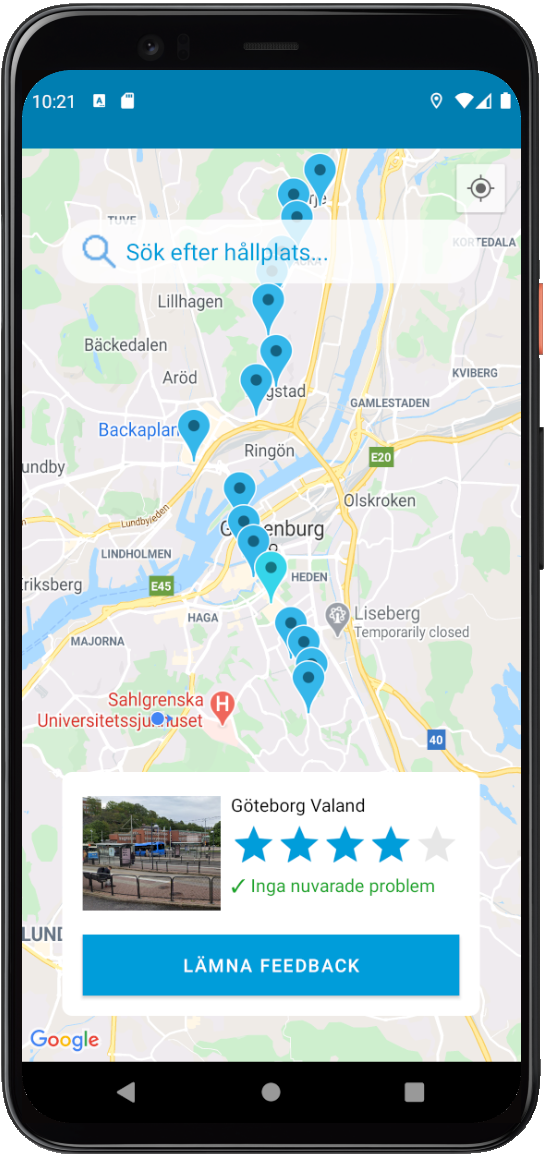
\includegraphics[width=.92\linewidth]{documentation/images/Info_card.png}
  \caption{Ett fönster med information om hållplatsen presenteras när en ikon väljs.}
  \label{fig:infofonster}
\end{minipage}%
\hfill
\begin{minipage}{.47\textwidth}
  \centering
  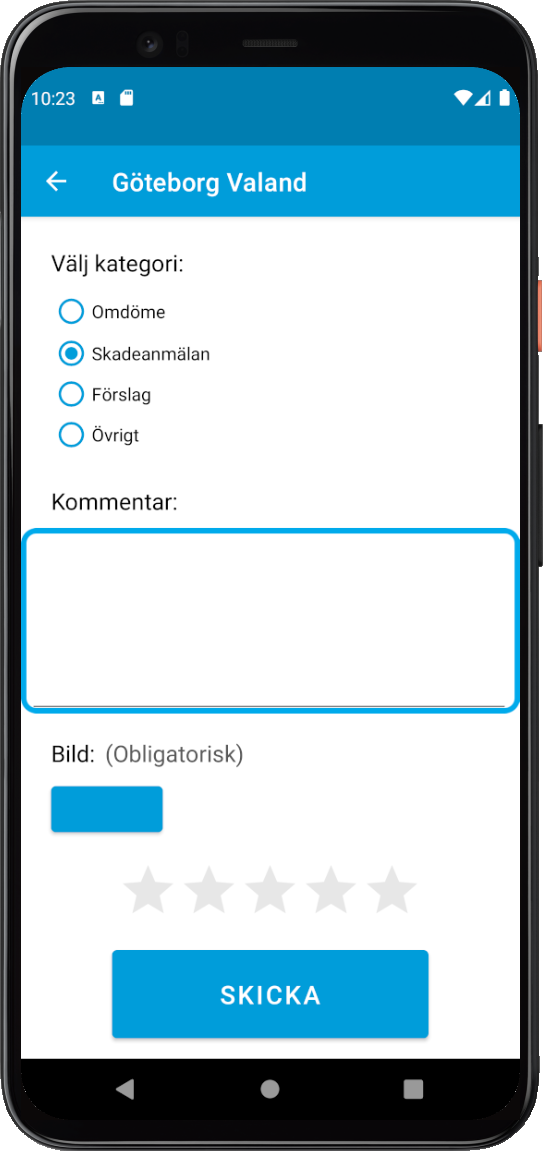
\includegraphics[width=.92\linewidth]{documentation/images/Feedback_screen.png}
  \caption{Sida där användaren kan lämna feedback för en hållplats. \\}
  \label{fig:feedbacksida}
\end{minipage}
\end{figure}

\section*{Applikationen}
\textit{Västtrafik Reviewer} är en app för att betygsätta och skaderapportera hållplatser runtom i Sverige. Appen presenterar en interaktiv karta över Sverige där användaren kan trycka på ikoner som representerar diverse hållplatser i landet. Genom att trycka på en av dessa ikoner visas ett fönster med namn och bild på hållplatsen samt genomsnittsbetyg och aktuell status, se figur \ref{fig:infofonster}. I fönstret kan användaren trycka på en knapp för att lämna en rapport om hållplatsen. På den sidan, figur \ref{fig:feedbacksida}, får användaren fylla i följande fält:
\begin{description}
\item[Kategori] \textendash\ vad för sorts rapport det är.
\item[Kommentar] \textendash\ kommentaren som användaren vill ge för platsen.
\item[Bild] \textendash\ om den valda kategorin är \textit{Skadeanmälan} tas en sådan på plats.
\item[Betyg] \textendash\ upp till fem stjärnor kan ges för platsen.
\end{description}

\subsection*{Målgrupp}
Appens målgrupp är individer som reser med buss och tåg. Då den erbjuder en organiserad, anonymiserad informationskälla kring dessa individers åsikter och förslag för specifika hållplatser gynnar den även Västtrafik. 

\subsection*{Avgränsningar}
Det fanns många potentiella funktioner som hade kunnat implementerats och som även togs upp. Däremot, på grund av tidsbegränsningar, exkluderades dessa funktioner. Funktioner som exempelvis \textit{inställningar} hade varit önskevärt för att erbjuda användaren större applikationsanpassning. Saker som olika färgteman och alternativa språk hade ökat tillgänglighetsaspekten av appen avsevärt. Dessutom fanns tekniska besvär som orsakade avgränsningar.
\\\\
Det var tänkt att alla hållplatser skulle hämtas från en API. Men nyckeln för att få tillgång till hållplatserna fungerade aldrig. Därför skapades istället en backend i programmet som innehåller ett antal hårdkodade hållplatser. 



\section*{Etik- och Hållbarhetsaspekter}
\subsection*{Sociala aspekter}
Genom att se till att göra hållplatser säkrare främjas, på ett sätt, den sociala aspekten med kollektivtrafik. Att västtrafik tillhandahåller ett medel för deras resenärer att kommunicera önskemål och åsikter till företaget kan anses som en social aspekt av hållbarhet. Detta för att appen försöker främja resenärers förhållande i trafiken.

\subsection*{Ekonomiska aspekter}
Eftersom den utmaning som gruppen valde hade centrum i trygghet inom kollektivtrafiken har fokus inte varit på att adressera den ekonomiska aspekten. Dock påverkas de ekonomiska aspekten på ett indirekt sätt. 
\\\\
Genom att det mer enkelt finns tillgång till en plattform där individer kan lämna ett förslag eller skadeanmälan på en specifik hållplats kommer det finnas mer feedback på de olika hållplatser. Med denna information kan man sedan lätt förbättra dessa platser. De resurser som då används för att reparera en eventuell skada eller en modifikation av en hållplats kommer i sitt sätt leda till en utveckling inom kollektivtrafiken.
\subsection*{Ekologiska aspekter}

Applikationens syfte är främst att få folk att tycka till om Västtrafiks hållplatser, och på så sätt få en säkrare och trevligare miljö kring hållplatser. Således är den ekologiska aspekten en mer indirekt konsekvens. Vid stort användande av applikationen bör det kollektiva resandet öka, och på så sätt minska hur många som åker bil. Detta i sin tur leder till en minskning av koldioxidutsläpp.
\\\\
Förutom ökat kollektivt resande kan det även leda till ekologisk hållbarhet på andra sätt, ponera till exempel att det kommer in mycket kommentarer om att en hållplats alltid är full av skräp. Det kan mycket väl visa sig att det inte finns någon soptunna i närheten av hållplatsen, vilket kanske inte hade upptäckts annars och skräpet hade hamnat i naturen. 
\\\\
På detta sätt finns även en direkt möjlighet för Västtrafik att arbeta för att inte bara göra deras resor mer ekologiskt hållbara, utan de kan även göra individuella hållplatser och knytpunkter mer ekologiskt hållbara. Denna klimatpåverkan må vara nästintill försumbar i jämförelse med klimatpåverkan av att fler åker kollektivt, men samtidigt har Västtrafik 21 000 hållplatser - så totalt sett borde det göra en skillnad, även om den inte är lika omfattande. 

\subsection*{Etiska aspekter}

Att skapa en app kommer inte utan utmaningar av olika slag. En aspekt man bör fundera över är funktionen för platsinformation som inte är helt oproblematisk utifrån ett etiskt synsätt. Enligt föreläsningen “Konsekvensetik” med Niklas Mörk ses en handling som moraliskt rätt eller fel beroende på konsekvensen av handlingen. Med detta synsätt kan platsinformation därför ses som både rätt och fel, beroende på vad utfallet blir. Å ena sidan blir appen mer lättanvänd vilket i längden kan medföra att upplevelsen av att resa kollektivt blir bättre, å andra sidan finns risk för att information missbrukas och konsekvensen av det skulle då kunna innebära integritetskränkning av användarna. Vissa människor kommer inte vilja använda sig utav platsinformation just på grund av risk för integritetskränkning och det kommer då bli svårare att använda appen eftersom den till viss del bygger på den funktionen. 
\\\\
Appen kommer förhoppningsvis öka benägenheten att vilja åka mer kollektivt då den är utformad på ett enkelt och användarvänligt sätt samt att den används för att skapa en bättre och tryggare miljö runt hållplatser och knutpunkter. Trafikverket: “Bland motordrivna färdmedel är tåg, buss och tunnelbana de mest miljövänliga energieffektiva alternativen, räknat per personkilometer.” Med tanke på den stora miljövänligheten för just kollektivtrafik påverkar appen hållbarheten i förlängningen, förutsatt att många människor kommer vilja använda den. 
\\\\
En ökad användning av kollektivtrafik är positivt för miljön men under pågående pandemi är denna typen av samlingar istället negativt ur en smittspridnings-aspekt. I föreläsningen “Miljöetik” ställer sig Martin Persson frågan: “Vems intressen räknas i hållbar utveckling?” och för vår app är samma frågeställning intressant. Vad är viktigast? Att resa mer kollektivt för att rädda de människor som om hundra år kan komma att lida av miljöförändringar till följd av nutida utsläpp, eller att begränsa resandet i kollektivtrafik för att minska smittspridningen av dödliga covid-19 och på så sätt rädda människoliv just nu? Utifrån ett antropocentriskt synsätt skulle det kunna vara det bäst att inte begränsa kollektivtrafiken eftersom mänskligheten i stort (inklusive de som ännu inte är födda) gynnas mer av fortsatt användande av kollektivtrafik och andra miljövänliga inslag som kan rädda vårt släkte och öka våra möjligheter här på jorden i framtiden. 
\\\\
Som Frances Sprei presenterade i föreläsningen om etik, definieras hållbar utveckling enligt Brundtland Report av World Commission on Environment \& Development, 1987: “Att möta dagens behov utan att kompromissa möjligheten att möta framtida generationers behov”.  
\\\\
Just nu är ett av våra behov att minska smittspridningen av pågående pandemi, men detta måste då alltså utifrån WCED:s syn på hållbarhet, göras utan att det påverkar våra möjligheter att möta framtida generationers behov. Där hamnar man i en rävsax då kollektivtrafiken är en stor samlingsplats för smitta men samtidigt en väldigt viktig del i hållbar utveckling som bidrar till att spara jordens resurser till kommande generationer och med andra ord ha möjligheten att möta deras behov. 
\\\\
\section*{Förbättringsområden}
\subsubsection*{Tillägga alla busshållplatserna: }
Den aktuella versionen av applikationen innehåller hållplatserna till linje 18. Nästa steg ska vara att tillägga resten av busshållplatserna.
\subsubsection*{Integrera med togo applikation: }
Ur användarens perspektiv anses Applikationen som komplettering tjänst till det huvud sakliga tjänst som är kollektivtrafik. Detta kan skapa svårighet att få stor antal användare. Lösning till detta kan vara att integrera vårt applikation med västtrafiks application"togo".
\begin{figure}[htp]
    \centering
    \includegraphics[width=4cm]{västtrafik}
    \label{fig:Map}
\end{figure}
\\\\
Hållplatserna presenteras som noder i togo applikation.När man tryckar på en node, så visar appen hållplats namn. Det kan görs istället är att visa en feedback sida när man tryckar på en hållplats. Detta kan fungera på samma sätt som användt i vårt app.
\subsubsection*{Poäng system: }
Att locka användaren att skriva en recension är på sig själv en utmaning, eftersom användaren inte får en direkt fördel genom att lämna in en utvärdering på en busshållplats. Genom att implementera ett poängsystem, kan vi uppmuntra användare att ladda ner och använda applikationen fortlöpande. Poängsystemet ger användaren fem poäng för en skadeanmäla som inkluderar en bild och kommentar, tre poäng för ett förslag och två poäng för ett omdöme. poäng som användaren samlar kan omvandlar till en reskassa. Detta kräver dock att ha en registrering system samt att ha en sida där man kan se sin aktuella samlade poänd och omvandla sina poäng till resekassa.

\section*{Egna lärdomar}
Genom projektet har gruppens medlemmar fått ökad förståelse av applikationsutveckling genom användandet av Android Studio, samt erhållit erfarenhet i att samarbeta när all kommunikation sker digitalt. Fastän \textit{Västtrafik Reviewer} är en prototyp och inte är i behov av användardata i lika stor utsträckning som för en eventuell fullständig version, har hänsyn tagits till vilken användardata som behövs samt till vilken grad denna data görs tillgänglig för övriga användare. Att till exempel göra användarens kommentarer synliga för andra skulle från andra användares synvinkel kunna ge bättre insikt till varför en hållplats har ett visst snittbetyg, men kan å andra sidan kan det beroende på innehåll offentliggöra personlig information samt öppna upp möjligheten till att lättare sprida felinformation. Dessa nackdelar kan motverkas genom att alla kommentarer passeras genom ett filter innan de görs tillgängliga till allmänheten, men implementeringen av denna är en etisk och teknisk utmaning i sig och faller utanför ramen för detta projekt.

\end{document}
